%%\documentclass[preprint,10pt]{sigplanconf}
%%\documentclass[10pt]{journal}
%%\documentclass[preprint, 10pt]{sigplanconf}



\documentclass{acm_proc_article-sp-sigmod09}

%%\usepackage{amsthm}


\usepackage{color}
\usepackage{times}
%%\usepackage{url}
%%\usepackage{graphicx}
%%\usepackage{boxedminipage}
\usepackage{xspace}
\usepackage{textcomp}
\usepackage{wrapfig}
%%\usepackage{verbatim}
%%\usepackage{latexsym}
\usepackage{amsmath, amssymb}
%%\usepackage{amsthm}


\newcommand{\jmh}[1]{{\textcolor{red}{#1 -- jmh}}}
\newcommand{\paa}[1]{{\textcolor{blue}{#1 -- paa}}}
\newcommand{\rcs}[1]{{\textcolor{green}{#1 -- rcs}}}
\newcommand{\nrc}[1]{{\textcolor{magenta}{#1 -- nrc}}}
\newcommand{\smallurl}[1]{{\small \url{#1}}}



\begin{document}
%
% --- Author Metadata here ---
\conferenceinfo{ACM PODS}{'10 Indianapolis, IN, USA}
%\setpagenumber{50}
%\CopyrightYear{2002} % Allows default copyright year (2002) to be over-ridden - IF NEED BE.
%\crdata{0-12345-67-8/90/01}  % Allows default copyright data (X-XXXXX-XX-X/XX/XX) to be over-ridden.
% --- End of Author Metadata ---

\title{Dedalus\titlenote{\small
Dedalus is intended as a precursor language for \textbf{Bloom}, a high-level language for programming distributed systems that
will replace Overlog in the \textbf{BOOM} project.  
As such, it is derived from the character Stephen Dedalus in James Joyce's \emph{Ulysses}, whose dense and precise chapters 
precede those of the novel's hero, Leopold Bloom.  The character Dedalus, in turn, was partly derived from Daedalus, the greatest
of the Greek engineers and father of Icarus.  Unlike Overlog, which flew too close to the sun, Dedalus remains firmly grounded.
}: 
Datalog in Space and Time} 
%%Format\titlenote{(Produces the permission block, copyright information and page numbering). For use with ACM\_PROC\_ARTICLE-SP.CLS V2.6SP. Supported by ACM.}}
%
% You need the command \numberofauthors to handle the "boxing"
% and alignment of the authors under the title, and to add
% a section for authors number 4 through n.

\numberofauthors{5}

\author{Peter Alvaro, Neil Conway, Tyson Condie, Joseph M. Hellerstein, David Meiers}
%%\author{Neil Conway}

\maketitle

\begin{abstract}
foo
\end{abstract}

\section{Introduction}

\subsection{Datalog}

\subsubsection{The basics}  

\subsubsection{Negation and stratification}

\subsubsection{Local stratification}

\subsubsection{Choice}

\subsection{Motivation: Distributed Systems}

Datalog is static.  What does Datalog even \emph{mean} extended in time?

Overlog pretended there was no time; we used the ``chain of fixpoints" model and treated the database as overwritable storage. 

\section{Dedalus}

By reifying time as data, we are able to reason about time in our logic.  some useful things fall out of this right away: persistence is now programatic rather than a separate type, ditto key constraints.  event creation vs. effect ambiguities are resolved.

Perhaps more importantly, the infinite sequence of abstract time gives us a way to reason about ordering, which is particularly difficult in a set-oriented language like Datalog.  The ordering over any program inputs (e.g. message queues) can be represented as a mapping between the ordering domain of the input and the time relation.

\subsection{Syntax}
\subsubsection{Events}
\begin{verbatim}
likes(peter, swimming)@123;
\end{verbatim}

\subsubsection{Persistence}

\begin{verbatim}
likes(Person, Activity)@N+1 :-
  likes(Person, Activity)@N,
  notin del_likes(Person, Activity)@N;
\end{verbatim}

or does this look better?

$
likes(Person, Activity)@N+1 \leftarrow \\
  \quad \quad likes(Person, Activity)@N, \\
  \lnot~del\_likes(Person, Activity)@N;
$

\subsubsection{State Change}

it appears that under this interpretation a database is an atomic (due to the adjacent timestamps)
pair of events with a deletion of the old value and assertion of the new, e.g.

$
del\_likes(peter, swimming)@456; \\
likes(peter, hiking)@457;
$

\subsubsection{Sequences}

$
seq(Agent, S + 1)@N+1 \leftarrow \\
  seq(Agent, S)@N, \\
  event(Agent)@N; \\
  \\
seq(Agent, S)@N+1 \leftarrow \\
seq(Agent, S)@N, \\
\lnot event(Agent)@N;
$

\subsection{Semantics}
\subsubsection{Chain of fixpoints interpretation}
\subsubsection{Instantaneous time interpretation}

\subsection{Examples}

\section{Equivalences}

\subsection{Dedalus is Datalog if we project out time}

\subsubsection{Theorem 1}

%%\begin{theorem}
\newtheorem{foo}{bar bas bat}
every local Dedalus program P with only deductive rules is equivalent to a Datalog program P'.
%%\end{theorem}

\subsubsection{Theorem 2}

every local Dedalus program P with deductive and inductive rules and trace T is equivalent to a Datalog program P' with an EDB T'.

\subsubsection{Theorem 3}

some theorem about distributed programs :)

\subsection{Dedalus programs are stratifiable if the equivalent Datalog program is stratifiable}

\subsubsection{Theorem 4}

\subsection{Space is simply time}

Dedalus programs can model many classes of distributed systems.  Take the (distributed) program

$
ping(@A, B)@N + r(A, B) \leftarrow \\
init(A, B)@N; \\
\\
pong(@B, A)@N + r(A, B) \leftarrow \\
ping(@A, B)
$

We may regard  \emph{r()} as a function over the attributes occurring in the body of the rule.  The implementation or \emph{r()} is provided by
the model.  For example:

\subsubsection{Synchronous Systems}

r(\_) = 1 for all \_.  Computation proceeds in rounds.

\subsubsection{Asynchronous Systems}

The return value of r may be any arbitrary integer, positive or negative, including a NULL integer indicating an infinite value.

\subsubsection{Lamport Clocks}

As a middle ground, we might wish to enforce a constraint that $r(\_) > 0$.  Doing so would entail implementing a \emph{Lamport Clock}.

\begin{figure}[t]
  \centering
  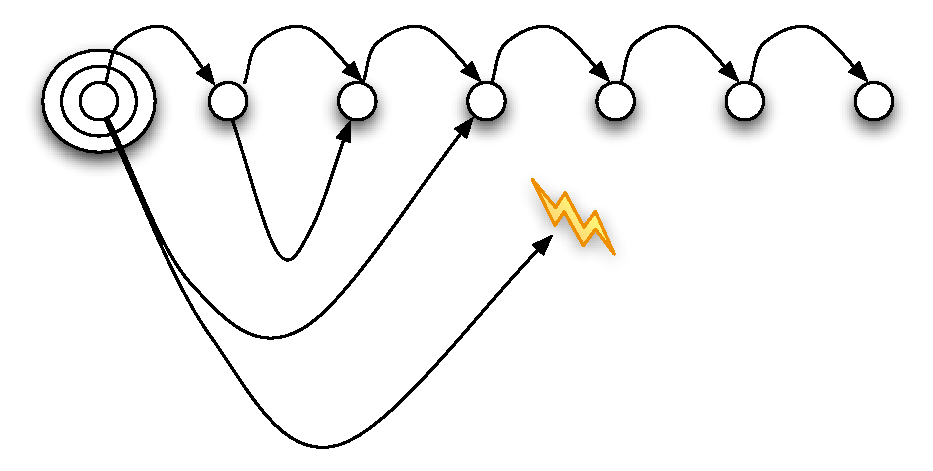
\includegraphics[width=0.75\linewidth]{dedalus-time.pdf}
  \label{fig:dedalus-time}
  \caption{Time moves forward in three ways: across strata, to the next fixpoint, and to some future fixpoint.}
\vspace{-8pt}
\end{figure}


\subsection{All sequence inputs are derived from time}

Input queues are simply a mapping between the ordering domain of the queue tuples and the time relation.  Naturally, this mapping
is infinite also and cannot be expressed as EDB.  But we can instead constructively state the rules that define how the mapping 
tracks the progress of the time relation.

\subsection{Dedalus Programs can be efficiently implemented}

:)

\subsubsection{Local stratification on time}

\subsubsection{Time is infinite but punctuated}

and indeed, so are any input streams.  we may dequeue as many events as we like from a given stream by using the mapping
between the elements in the queue and the time relation.  in the simplest case this mapping would be from the ordering domain 
of the queue to the time domain, but we can establish more complicated data-dependent mappings by including other attributes 
(e.g. we could implement QoS by including the address in the mapping and dequeueing a different number of items per host
per time unit).

\subsection{Dedalus Programs are storage-optimal}

:)

\subsubsection{We need only store the event tuple with max(Timestamp) for each projection of the other columns to query the present time}


\subsubsection{perhaps we can admit queries over the past that are bounded and pre-stated, and do GC}

\section{Correctness properties}

\subsection{Safety}

we need merely to show the base case, in which an invariant is established (in fact, this should \emph{always} be a valid 
initial state, or the safety property isn't guaranteed to always hold), the existence of an inductive rule that ensures that every 
subsequent step maintains the invariant, and the absence of any rule that can break the induction by deducing a del\_* rule.

\subsection{Liveness}

We cannot state a liveness property as an assertion, because doing so would involve quantifying over time,
and time is an infinite sequence.  Instead, we must prove liveness properties, expressed as temporal logic
formulae, given the rules of the program and any given safety properties as axioms.

In many cases it will be possible to show that attempts to achieve liveness properties will occur infinitely often, and that
these attempts have a nonzero probability of success.  We'd like to do better than this and provide realistic guarantees...

\subsubsection{Deadlock}



\subsubsection{Livelock}

\subsection{Examples}

\section{Future Work}

%%\bibliographystyle{abbrvnat}
%%\bibliography{eurosys}

%%\section{Proof of Lemma 1}
\begin{proof}
%First, we prove an isomorphism between stable models, and finite prefixes of stable models.  Scan a stable model of a program timestamp by timestamp.  
We first present an algorithm for computing ultimate models, and argue that the algorithm computes exactly the ultimate models of the \lang program.  We then argue this algorithm can be run on our operational formalism, and show how operational traces correspond with prefixes of stable models.

Any \lang program without asynchronous rules is a $\text{Datalog}_{1S}$ program, and the algorithm given in~\cite{tdd} computes its ultimate model in polynomial space\footnote{The class of {\em multi-seperable}~\cite{tdd-poly} \lang programs, which comprises all \lang programs $P$ with guarded asynchrony and persisted EDB, and their coordinations $\textsc{Coord}(P)$, can be executed in polynomial time in the size of the input.} in the size of the input.  The algorithm evalutes the program for $2^G + e$ consecutive timesteps, where $G$ is the number of instantiations of the non-temporal attributes of the program rules using all combinations of constants in the Herbrand Universe, and $e$ is the maximum timestamp of any EDB fact.  At each step, the algorithm updates information on observed periodicities of facts.  When the algorithm terminates, any fact with a periodicity of 1 is regarded as part of the ultimate model.

For asynchronous rules, the natural distributed analog of the above algorithm simultaneously executes one instance for each node \dedalus{n}, using values of $G$ and $e$ computed from $E_{\text{\dedalus{{\scriptsize n}}}}$.  Each instance has its own local clock, which corresponds to the timestamp attribute in the model-theoretic semantics.  Nodes communicate over channels with arbitrary delay and message re-ordering.  When a remote node \dedalus{m} derives a fact at \dedalus{n}, it encloses its local clock value, \dedalus{t}; \dedalus{n} must consider this fact at his local time \dedalus{t} or later, in the style of Lamport Clocks.  Note that this behavior is equivalent to the model-theoretic semantics of remote asynchronous rules: remote deductions are visible at the destination at a time later than the body temporal attribute at the source.  Further, note that Lamport Clocks only introduce the constraint that if message $a$ ``happens before'' $b$, in other words $a$ directly or transitively causes $b$ to be sent, then $T(a) < T(b)$.  If $a$ and $b$ are concurrent, there is some execution where $T(a) \geq T(b)$.

When \dedalus{n} processes a received message, the number of constants available to \dedalus{n} may increase, and thus the node's $G$ may increase to $G'$.  Furthermore, the node may need to execute over this new fact for $2^{G'}$ additional timesteps.  If only finitely many messages are sent, this algorithm terminates, and requires polynomial space.  In the case that infinitely many messages are sent, we only need to process each message $2^{G'}$ times: the maximum period of any fact is $2^{G'}$, as every incoming fact needs to have a chance (in some execution) to join with any deduction (with which it is ``concurrent'') at any time during its period.  Keeping track of the number of times we have seen each fact also requires polynomial space.  When the algorithm is done running for $2^{G'}$ steps, it pauses, waiting for new network input that it has not seen enough times.  If all nodes are paused and no outstanding messages exist, then the collection of all period 1 facts at all instances of the algorithm comprises an ultimate model.

We claim that the algorithm can generate every ultimate model---every message has the opportunity to join with another concurrent message or its transitive consequents at any point during their period, and has the opportunity to join with a causally related message during the range of times allowed by the model-theoretic constraint (identical to the Lamport Clock condition used in the algorithm).  Furthermore, the set of all facts, and their local timestamps, comprises a prefix of a stable model.

Note that we can execute this algorithm straightforwardly on our operational formalism.  Evaluating a single timestamp of a \lang program corresponds to the evaluation of a Datalog program, which is a polynomial time computation, and the Turing Machines can also maintain the necessary state about periods and message counts.
%2) Intuitively, the operational model is based on n Turing Machines, one per value of node(), which independently step sequentially through time and communicate via channels with
%non-deterministic delay.  At each timestep t they run a datalog fixpoint computation that evaluates P on ``projection(E_n, t)'' (notation needed); this takes polynomial
%time~\cite{immerman}.  At the end of this fixpoint there are three sets of relevant facts: local, synchronous facts that have timestep t+1 and become part of ``projection(E_n,
%t)'', local asynchronous facts whose timestep is chosen non-deterministically to be greater than t and become part of later timesteps, and remote asynchronous facts.  The
%timestamps in this third class of facts are chosen non-deterministically ``at the receiver'' to model delay, in a way that observes traditional causality
%restrictions~\cite{lamportclocks}.
%3) Any \lang program without  async rules is a Datalog_{1S} program, and the above intuition is captured by the algorithm given in~\cite{}, computing an ultimate model in
%polynomial space in the size of the input.  In the presence of asynchronous rules, this formalize needs to be expanded to account for the asynchronous advancement of time through
%\dedalus{successor} at each node.  The PSPACE guarantees of~\cite{} are not shown to hold for such programs, but in Appendix Foo we show that the following Lemma holds for all
%\lang programs under this model
\end{proof}

\section{Proof of Lemma 2}
\begin{proof}
We begin by assuming that \dedalus{node} contains the identifiers of each of the $n$ nodes.  Since the atemporal fragment of \lang is FO[LFP], we can represent a polynomial-time bounded Turing Machine using only atemporal rules in \lang~\cite{immerman-ptime}.  In addition to normal operations, the Turing Machine can place items into a queue---\cite{dedalus} shows how to model queues in \lang---or send messages to other nodes---modeled by an asynchronous communication rule with \dedalus{queue} in the head.  A node persists the contents of the tape across time if the queue is empty, using a rule like \dedalus{tape(\dbar{X})@next <- tape(\dbar{X}), !queue(\dbar{\_});}.  If the queue is non-empty, the computation skips a timestamp (leaving \dedalus{tape} empty), and then atomically copies the contents of \dedalus{queue} to \dedalus{tape}.  The ultimate model of this program is exactly the final contents of the tape on every node if the computation halts.  Otherwise, the program's ultimate model is empty: \dedalus{tape} facts only exist every other timestamp, and for any Turing Machine predicate \dedalus{r} we can create \dedalus{r'}, and create a mutual recursive cycle to ensure neither \dedalus{r} nor \dedalus{r'} contains facts at every timestamp:

\begin{Dedalus}
r(\dbar{X})@next <- r'(\dbar{X});
r'(\dbar{X})@next <- r(\dbar{X});
\end{Dedalus}

We can play a somewhat similar trick for \dedalus{queue} by having local messages alternate between going into \dedalus{queue} and \dedalus{queue'}.  Thus, no local queue message will be part of the ultimate model.  Remote messages will still go into \dedalus{queue}: this still leaves the case that the exact same message repeatedly arrives at a node at every timestamp forever, by chance.  We can dispense of this case by assuming the channels interconnecting the Turing Machines forbid it.
\end{proof}

\section{Proof of Lemma 3}
\begin{proof}
Our proof proceeds via construction of a two counter machine in \lang, inspired by the construction in~\cite{undecidable-datalog}.

We represent the state of a two counter machine using the \linebreak \dedalus{cnfg(T,S,C1,C2)} relation, where \dedalus{T} represents ``time'' (note this is not the same as the \lang temporal attribute), \dedalus{S} is the state, and \dedalus{C1} and \dedalus{C2} are the values of the two counters.  In order to support our two instructions, $inc$ and $dec$, we would like to make use of the \dedalus{successor} relation.  However, \lang conventions forbid the use of this infinite relation outside of the timestamp attribute.  Thus, we posit the \dedalus{fin\_succ(X,Y)} EDB relation, which is meant to represent a finite prefix of the \dedalus{successor} relation.  Since it is EDB, its contents may be arbitrary.  If \dedalus{fin\_succ} is malformed, then the machine's execution may be incorrect.  In particular, our model of the machine may accept an input, whereas the actual machine would not have accepted that input.  We illustrate how to constrain the contents of \dedalus{fin\_succ} below:

\begin{Dedalus}
malformed() <- fin_succ(_,0);
malformed() <- fin_succ(X,Y), fin_succ(X,Z), Y != Z;
malformed() <- fin_succ(Y,X), fin_succ(Z,X), Y != Z;
malformed() <- fin_succ(X,Y), X >= Y;
\end{Dedalus}

For a given EDB, the two counter machine either halts in the accepting state or halts in a non-accepting state.  It cannot run forever since the EDB (in particular, the \dedalus{fin\_succ} relation) is finite.

We construct a \lang program that nondeterministically decides to either run the machine on the input provided (and for the length of \dedalus{fin\_succ} provided, or declare that the machine will never accept without running it.  If the machine ever accepts some input, this induce two different ultimate models---one generated by a trace where we run the machine and it accepts, and one generated by a trace where we decide to not run the machine, and thus we implicitly reject.  We describe the program below. 

Initially, we nondeterministically decide whether to run the machine or not by sending two messages (0 and 1) to a remote node (\dedalus{decider}).  If both message arrive simultaneously, then the decider responds to run the machine.  Otherwise, the decider responds to declare failure:

%\jmh{should we use a hashmark for constants?  I would say no.}
\begin{Dedalus}
//send two messages to the decider
message(#D, 0)@async <- decider(D);
message(#D, 1)@async <- decider(D);

//decider responds to computer
run_machine(#computer)@async <- message(0),
                                message(1);
declare_failure(#computer)@async <- message(0),
                                    !message(1);
declare_failure(#computer)@async <- !message(0),
                                    message(1);
\end{Dedalus}

Each mapping in the transition function is expressed by a \lang rule with \dedalus{!malformed()} and \dedalus{!declare\_failure()} in its body.  For example, the rule $\delta(3, > =) = (7, inc, dec)$ would be represented as:

\begin{Dedalus}
cnfg(S,7,D1,D2) <- cnfg(T,3,C1,C2), C1 > 0, C2 == 0,
                   fin_suc(T, S), fin_succ(C1, D1),
                   fin_succ(D2, C2), !malformed(),
                   !declare_failure();
\end{Dedalus}

We declare success or failure as follows:

\begin{Dedalus}
reject() <- !accept();
accept() <- cnfg(20,_,_); //20 is the accepting state
accept()@next <- accept();
\end{Dedalus}

If we choose to declare failure, or the machine halts in a non-accepting state---whether it is due to incompleteness or malformedness of \dedalus{fin\_succ}, or actual halting---then the ultimate model will contain \dedalus{reject}.  If the machine halts in an accepting state, then the ultimate model will contain \dedalus{accept}.  Thus, if we can decide confluence of this program, then we can decide whether there is any input for which an arbitrary two-counter machine halts.
\end{proof}


\end{document}
